% Section 2.1: Gamma-Ray Production Mechanisms
% Structure: Introduction -> Hadronic -> Leptonic -> GDE Model

\section{Gamma-Ray Production Mechanisms}
\label{sec:production_mechanisms}

% Before cataloging individual point sources or attempting to extract information from the faint extragalactic emission, one must understand the physical processes that generate \blue{the intense Galactic foreground introduced above}.

This section reviews the standard gamma-ray production mechanisms responsible for the Galactic diffuse gamma-ray emission.
These processes fall mainly into two broad categories: hadronic interactions involving cosmic-ray nucleons colliding with interstellar gas, and leptonic interactions involving energetic electrons and positrons scattering off radiation fields and gas.
% Operating in different energy regimes and tracing distinct target environments, they combine to produce the macroscopic Galactic Diffuse Emission that dominates the observed gamma-ray sky.

\blue{Both families of processes operate within the \emph{interstellar medium} (ISM), the mix of gas, dust, radiation, magnetic fields, and cosmic rays that fills the space between stars.
The ISM is mainly made of gas---roughly three-quarters hydrogen and one-quarter helium, with heavier elements and dust particles together contributing less than a percent. }
% It is organized into several coexisting phases spanning a wide range of temperature and density: cold molecular clouds in which hydrogen is bound into H$_2$; a neutral atomic medium traced by the 21 cm line of H\,\textsc{i}; and ionized phases (H\,\textsc{ii}), photoionized by stellar radiation and shock-heated by supernovae.
\blue{This gas supplies the collision targets for the hadronic interactions and bremsstrahlung discussed below, while the \emph{interstellar radiation field}---starlight, infrared emission, and the CMB---provides the seed photons for inverse Compton scattering.	}

\subsection{Hadronic Emission}
\label{sec:hadronic}

High-energy cosmic-ray protons and heavier nuclei interact with the interstellar medium through the strong nuclear force, primarily colliding with ambient hydrogen gas.
These inelastic proton-proton collisions produce secondary particles, most notably pions: 
\be
 p + p \to \pi^0 + \pi^{\pm} + X.
\ee
The reaction is subject to a strict kinematic threshold.
A cosmic-ray proton colliding with a stationary target proton must have a total energy of at least $E_p > m_p + 2m_\pi + m_\pi^2 / 2m_p \approx 1.2$ GeV in order to produce one or more pions \cite{Hooper:2024}.
Once this threshold is crossed, the total inelastic cross section increases only mildly with energy, rising from $\sigma_\text{inel}^{pp} \approx 30$--$40$ mb at $E_p \lesssim 10$ GeV to $\sigma_\text{inel}^{pp} \approx 100$ mb near $E_p \sim 1$ EeV \cite{Hooper:2024}.
Because a significant fraction of the proton's kinetic energy is transferred in each collision (inelasticity $K_{pp} \sim 0.5$), only a few successive interactions suffice to extract most of the cosmic ray's original energy \cite{Dermer:2009zz}.

\begin{figure}[t]
	\centering
	% Note: Using Kafexhiu et al. (2014) Figure 13 (right panel) as CC-licensed replacement
	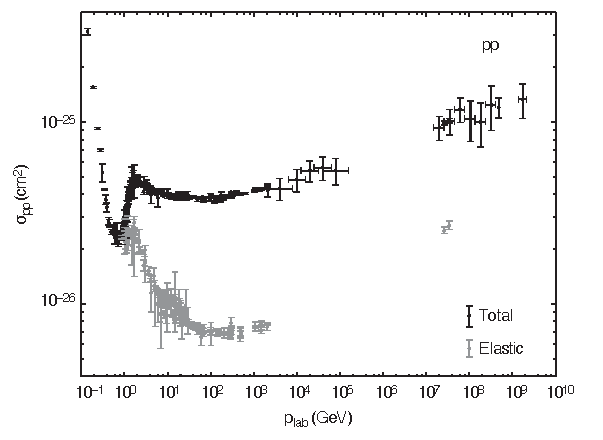
\includegraphics[width=0.7\columnwidth]{figures/sigma_pp.pdf}
	% \caption{Inclusive $\pi^0$ production cross section for inelastic proton-proton collisions as a function of the incident proton energy.
	% 	Different theoretical models (Geant4, Pythia8, QGSJET, SIBYLL) diverge at extremely high energies but provide consistent predictions across the primary cosmic-ray regime.
	% 	Credit: Figure 13 from Kafexhiu et al.\ (2014) \cite{Kafexhiu:2014cua}.
	% 	\aure{replace this with a pp cross section to show the pion bump, maybe}
	% }
	\caption{\blue{Measurements of the total and inelastic proton-proton cross section, where the so-called pion bump is clearly visible. Adapted from \cite{ParticleDataGroup:2022pth}.}}
	\label{fig:pp_cross_section}
\end{figure}

While charged pions ($\pi^\pm$) decay into muons and neutrinos, neutral pions decay electromagnetically with a mean lifetime of only $\tau_{\pi^0} \approx 8.4 \times 10^{-17}$ s: 
\be
 \pi^0 \to \gamma\gamma.
\ee
In the rest frame of the $\pi^0$, this decay produces two photons of equal energy $E_\gamma = m_{\pi^0}/2 \approx 67.5$ MeV.
In the laboratory frame, however, a pion moving with energy $E_\pi$ generates a gamma-ray spectrum that is flat between the kinematic bounds $(E_\pi - \sqrt{E_\pi^2 - m_\pi^2})/2$ and $(E_\pi + \sqrt{E_\pi^2 - m_\pi^2})/2$, and vanishes outside this interval \cite{Hooper:2024}.
This flat distribution has a remarkable consequence: regardless of the spectral shape of the parent pion population, the resulting gamma-ray spectrum---when plotted as $E^2 \, dN/dE$---always peaks at $m_{\pi^0}/2 \approx 67.5$ MeV.
This universal spectral feature, known as the \emph{pion bump}, is the definitive spectral signature of hadronic cosmic-ray interactions with gas and has been conclusively observed in both supernova remnants and the Galactic Plane emission \cite{Fermi-LAT:2013iui}, see Figure~\ref{fig:pp_cross_section}.
% Figure~\ref{fig:pp_cross_section} shows the inclusive $\pi^0$ production cross section as a function of proton energy across the primary cosmic-ray regime; the parametrization of Kafexhiu et al.\ \cite{Kafexhiu:2014cua} is widely adopted in current gamma-ray analyses.

Hadronic emission dominates the Galactic Diffuse Emission along the Galactic Plane, where the column density of interstellar gas is highest.
As a result, it constitutes the primary astrophysical background for any dark matter search targeting the inner Galaxy\blue{, with consequences we quantify in Section~\ref{sec:gde_model}}.
While hadronic emission dominates wherever gas is abundant, leptonic processes---inverse Compton scattering, bremsstrahlung, and synchrotron radiation---provide the complementary diffuse components, particularly at high Galactic latitudes.

\subsection{Leptonic Emission}
\label{sec:leptonic}

Relativistic electrons and positrons produce high-energy photons through three primary mechanisms: inverse Compton scattering, bremsstrahlung, and synchrotron radiation.
These processes operate across different energy regimes and target environments, and their relative importance depends on the local astrophysical conditions along each line of sight.

\textbf{Inverse Compton scattering.}
Relativistic electrons can up-scatter low-energy ambient photons---the Cosmic Microwave Background (CMB), infrared dust emission, and starlight---into the X-ray and gamma-ray bands \cite{Blumenthal:1970gc}.
The behavior of this process depends critically on the ratio of the electron energy to the target photon energy $\epsilon$.
In the Thomson regime ($E_e \ll m_e^2/\epsilon$), a given electron up-scatters photons to a maximum energy of $E_\gamma^\text{max} \approx 4\epsilon E_e^2 / m_e^2$.
The quadratic dependence on $E_e$ implies that higher-energy electrons are vastly more efficient radiators, which steepens the resulting photon spectrum relative to the parent electron population.
Quantitatively, a power-law electron spectrum with index $\alpha$ ($dN_e/dE_e \propto E_e^{-\alpha}$) produces a gamma-ray spectrum with a softer index $-(\alpha+1)/2$ \cite{Hooper:2024}.
In this regime, the ICS energy loss rate takes a form mathematically identical to that of synchrotron radiation: 
\be
	\left.\frac{dE_e}{dt}\right|_\text{ICS}^\text{Thomson} = -\frac{4}{3}\,\sigma_T\,\rho_\text{rad}\,\gamma_e^2\,c,
\ee
where $\rho_\text{rad}$ is the energy density of the target photon field \cite{Hooper:2024}.

\begin{figure}[t]
	\centering
	% adapted from Figure 5.1 from Hooper (2024)
	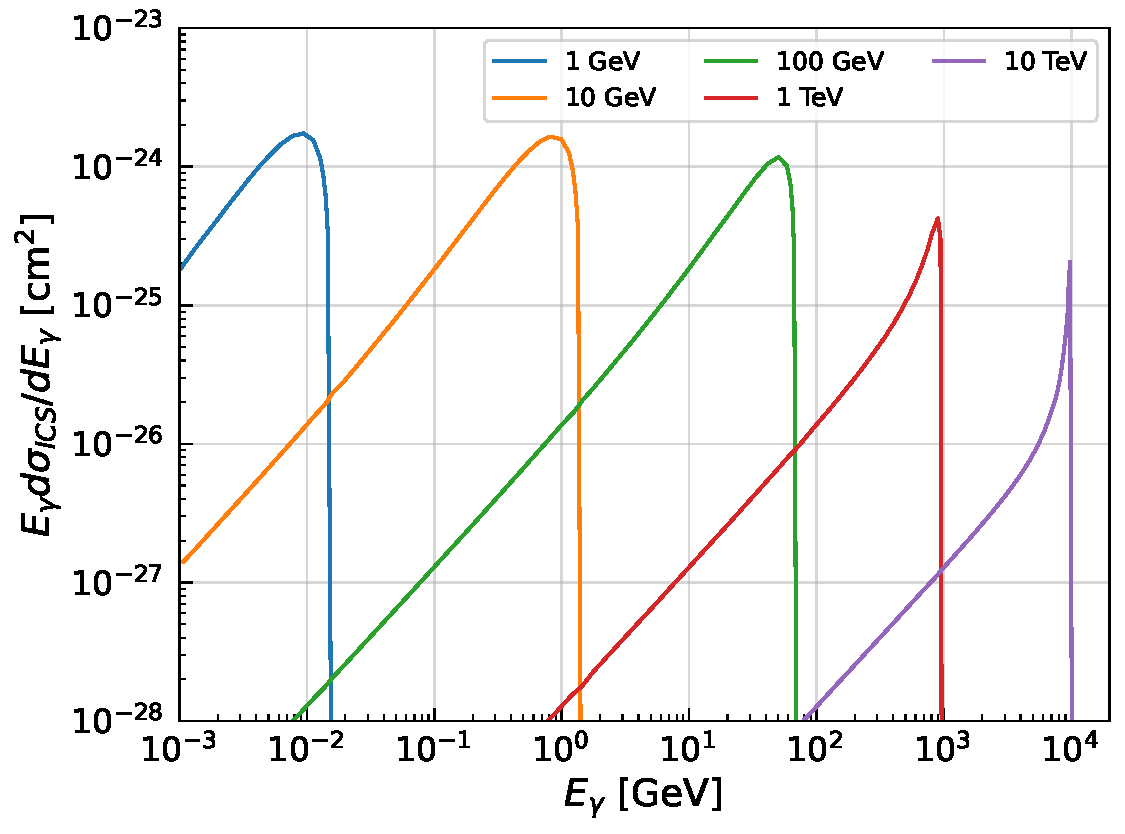
\includegraphics[width=0.7\columnwidth]{figures/ics-spectrum.pdf}
	\caption{The differential cross section for inverse Compton scattering of a high-energy electron with a 1 eV target photon, for several values of $E_e$.
		At high energies ($E_e \gg m_e^2/\epsilon$), the process enters the Klein-Nishina regime: the cross section is severely suppressed and the scattered photon carries nearly all the electron's energy.
	}
	\label{fig:ics_cross_section}
\end{figure}

At highly relativistic energies ($E_e \gg m_e^2/\epsilon$), the interaction transitions into the Klein-Nishina regime \cite{Hooper:2024}.
Here the scattering cross section drops below the Thomson value, and the energy loss rate acquires an additional suppression factor of $\sim m_e^4 / (E_e^2 T^2)$ relative to the Thomson prediction, where $T$ is the effective temperature of the target radiation field.
Consequently, the scattered gamma rays carry away nearly all the incoming electron's energy ($E_\gamma \approx E_e$), and the differential cross section peaks sharply just below $E_e$ rather than being spread across a broad range.
This transition from the Thomson to the Klein-Nishina regime is illustrated in Figure~\ref{fig:ics_cross_section}.

In practice, cosmic-ray electrons scatter off starlight, infrared dust emission, and the CMB.
At higher electron energies, Klein-Nishina suppression progressively reduces the efficiency of scattering off higher-frequency photons, shifting the dominant ICS target toward the CMB \cite{Hooper:2024}.

\textbf{Bremsstrahlung.}
In gas-rich regions of the interstellar medium, electrons undergo
bremsstrahlung as they decelerate in the Coulomb fields of neutral and ionized atomic gas.
The bremsstrahlung cross section scales with the square of the target nuclear charge ($\propto Z^2$), and hydrogen and helium are the dominant targets in the ISM.
A distinctive feature of bremsstrahlung is that its energy loss rate scales linearly with the electron energy at leading order ($b_\text{brem} \propto E_e$) \cite{Pinetti:2021jjs}, resulting in an energy loss timescale that is effectively independent of $E_e$.
As a consequence, the gamma-ray spectrum produced through bremsstrahlung closely mirrors the spectral shape of the parent electron population \cite{Hooper:2024}.
This process serves as the dominant cooling mechanism for cosmic-ray electrons in the MeV to GeV range in gas-dense environments such as the Galactic Plane, though it is broadly subdominant to hadronic emission in the same regions.

\textbf{Synchrotron radiation.}
In the presence of the Galactic magnetic field ($B \sim$ few $\mu$G), ultra-relativistic electrons gyrate around magnetic field lines and emit synchrotron radiation.
This process primarily generates photons in the radio and microwave bands, but it traces the same underlying electron populations that produce gamma rays via ICS and bremsstrahlung.
The synchrotron energy loss rate scales as $b_\text{syn} \propto B^2 E_e^2$ \cite{Hooper:2024}, mirroring the $E_e^2$ dependence of Thomson-regime ICS.
Which of the two mechanisms dominates depends on the local ratio of magnetic field energy density to radiation field energy density ($\rho_\text{mag}/\rho_\text{rad}$).
At the highest electron energies, Klein-Nishina suppression of ICS breaks this symmetry: the ICS loss rate falls below its Thomson-regime prediction, leaving synchrotron radiation as the primary cooling channel for the most energetic cosmic-ray electrons \cite{Hooper:2024}.

These three leptonic processes, together with the hadronic pion-decay mechanism described in the preceding section, constitute the main set of fundamental interactions that generate the diffuse gamma-ray sky.
The following section describes how these individual components are combined into a global model of the astrophysical Galactic Diffuse Emission.

\subsection{The Galactic Diffuse Emission Model}
\label{sec:gde_model}

The individual production mechanisms described in the preceding sections combine to produce the Galactic Diffuse Emission (GDE)---the brightest feature in the gamma-ray sky, accounting for roughly 80\% of all photons detected by the \textit{Fermi}-LAT \cite{Fermi-LAT:2014ryh,DGRB-review}.
This emission arises from the integrated interactions of propagating cosmic rays with the interstellar gas and radiation fields of the Milky Way.

To model this complex, spatially structured foreground, astrophysicists rely on numerical cosmic-ray propagation codes, of which GALPROP is one of the most established \cite{Strong:2007nh}.
Starting from a set of assumptions about cosmic-ray source distributions (primarily supernova remnants), injection spectra, and diffusion parameters, GALPROP solves the steady-state diffusion-loss equation for all relevant cosmic-ray species as they propagate through the Galactic magnetic field and interstellar medium.
The output is a set of sky maps predicting the gamma-ray intensity from each emission component: a $\pi^0$-decay map that traces the gas column density (dominated along the Galactic Plane), an inverse Compton map that traces the interstellar radiation field (producing an extended halo at high latitudes), and a bremsstrahlung map that follows the gas distribution but with a different spectral shape.

The resulting spatial and spectral morphology is highly structured and energy-dependent.
Along the Galactic Plane, where atomic and molecular gas is dense, hadronic pion decay dominates the high-energy emission, while bremsstrahlung and ionization govern the cooling of low-energy cosmic-ray electrons.
At high Galactic latitudes, the gas density drops while the interstellar radiation field remains significant.
There, inverse Compton scattering overtakes bremsstrahlung as the dominant energy-loss mechanism for electrons above a few tens of MeV, producing an extended, diffuse gamma-ray glow \cite{Pinetti:2021jjs}.
% The energy- and position-dependent balance between these loss channels is shown in Figure~\ref{fig:energy_loss_coefficients}.

% \begin{figure}[t]
% 	\centering
% 	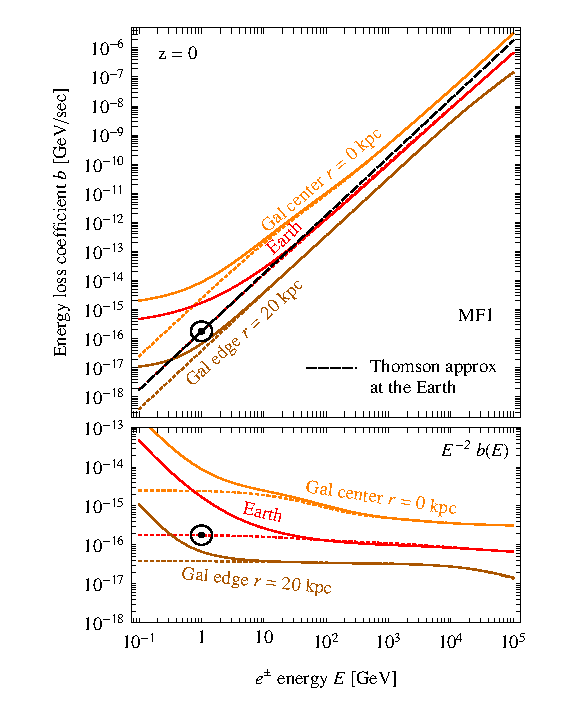
\includegraphics[width=0.7\columnwidth]{figures/energy_loss_coefficients.pdf}
% 	\caption{Energy loss coefficient function for electrons and positrons in the Milky Way's galactic disk at various radial distances from the Galactic Center.
% 		In the gas-rich Plane, ionization and bremsstrahlung dominate at low energies; at higher energies, inverse Compton scattering and synchrotron radiation become the primary loss channels. The transition to the Klein-Nishina regime suppresses the ICS efficiency at the highest energies, causing deviations from the Thomson approximation.
% 		Credit: Figure 7.1 from Cirelli et al.\ (2024) \cite{Cirelli:2024ssz}.
% 	}
% 	\label{fig:energy_loss_coefficients}
% \end{figure}

When analyzing \textit{Fermi}-LAT data, the standard procedure is to model the observed sky through template decomposition \cite{Fermi-LAT:2014ryh}.
The total photon counts in each spatial and energy bin are fit to a linear combination of: the GALPROP-derived $\pi^0$-decay, ICS, and bremsstrahlung templates; a catalog of individually resolved point sources; spatial templates for large-scale structures such as Loop I and the Fermi Bubbles; and a spatially uniform isotropic component representing the combined extragalactic background and residual instrumental contamination.
The normalizations of these Galactic templates are typically left as free parameters and fitted independently in each energy bin, allowing the data to correct for imperfections in the GALPROP predictions.
The Fermi collaboration applies precisely this procedure to produce the \blue{latest} official Galactic interstellar emission model \texttt{gll\_iem\_v07}, which serves as the standard foreground template in Fermi-LAT analyses.
\blue{One subtlety is worth flagging: in \texttt{gll\_iem\_v07} the Fermi Bubbles and Loop~I are not modeled from dedicated physical templates but absorbed into an \emph{ad hoc} component---the \emph{patch}---built by smoothing the large-scale residuals left over after the physical templates are fit, and adding them back into the model \cite{Fermi-LAT:2019yla,Fermi-LAT:2022byn}.
Since the patch soaks up any extended residual, including the Galactic Center Excess, the official Pass~8 models are by construction ill-suited to extended-emission studies---a caveat we return to in Chapter~\ref{ch:4}.}
Despite the physical sophistication of GALPROP and the flexibility of the template-fitting procedure, the GDE cannot currently be modeled perfectly.
Imperfect modeling of the interstellar emission remains the largest single source of systematic uncertainty in gamma-ray astrophysics, introducing errors between 15\% and 30\% depending on the energy range \cite{Fermi-LAT:2014ryh,DGRB-review}.
Uncertainties in the gas column densities (particularly the conversion from CO emission to molecular hydrogen), the interstellar radiation field, and the cosmic-ray propagation parameters all contribute.
Handling the Galactic foreground properly is a necessary condition for any analysis of the gamma-ray sky: without adequate foreground control, both spectral characterization and source detection are biased.
This challenge recurs throughout this thesis---in the extraction of the Galactic Center Excess (Chapter~\ref{ch:4}), the search for dark matter subhalos (Chapter~\ref{ch:5}), and the reconstruction of the extragalactic source-count distribution (Chapter~\ref{ch:6}).
The probabilistic and simulation-based methods developed in later chapters are designed to operate robustly in the presence of these foreground uncertainties, rather than to eliminate them.
